\documentclass[final]{beamer}

\usefonttheme[onlymath]{serif}
\usepackage[orientation=landscape, size=a0]{beamerposter}
\usepackage[absolute, overlay]{textpos}
\usepackage{tikz}

\usepackage{subfig}
\usepackage[export]{adjustbox}
\usepackage{float}

\usepackage{multirow}
\usepackage[default]{cantarell}
\usepackage[T1]{fontenc}
\usepackage{multirow}
\usepackage{color, colortbl}
\definecolor{darklavender}{RGB}{85, 63, 144}
\usepackage[percent]{overpic}
\setbeamertemplate{itemize item}{\raisebox{0.1ex}{$\blacktriangleright$}\hskip0.1em}
\usepackage{algorithm,algorithmic}

\usepackage{calc}

\newcommand{\embl}[1]{\textbf{\textcolor{blue}{#1}}}

\newcommand{\Tstrut}{\rule{0pt}{2.5ex}} % = `top' strut
\mode<presentation>
{
  \usetheme{default} % or try Darmstadt, Madrid, Warsaw, ...
  \usecolortheme{rose} % or try albatross, beaver, crane, ...
  \usefonttheme{default}  % or try serif, structurebold, ...
  \setbeamertemplate{navigation symbols}{}
  \setbeamertemplate{caption}[numbered]
  \setbeamertemplate{frametitle}[default][center]
  \setbeamerfont{frametitle}{size=\Large}
}

\usepackage[english]{babel}
\usepackage[utf8x]{inputenc}
\usepackage{xcolor}

\newenvironment<>{titleblock}[1][]{%
%  \setbeamercolor{block title}{fg=darklavender, bg=white}
  \setbeamercolor{block body}{fg=darklavender, bg=white}
}

\setbeamercolor{block title alerted}{fg=black, bg=white}
\setbeamercolor{block body alerted}{fg=black, bg=white}

\setbeamercolor{block body}{fg=black, bg=white}

\makeatletter
\newcommand\HUGE{\@setfontsize\Huge{70}{80}}
\makeatother  

\title{Test}

\captionsetup[subfloat]{labelformat=empty}

\newenvironment{myblock}[1]{\begin{block}{\centering \LARGE \textbf{#1}}}{\end{block}}

\newcommand{\placeholder}[2]{\\ (placeholder) \textcolor{gray}{\rule{#1}{#2}}}

\begin{document}

\addtobeamertemplate{headline}{} 
{
\begin{tikzpicture}[remember picture, overlay] 
\node [shift={(-11cm,-3cm)}] at (current page.north east) {
\includegraphics[scale=1.00]{uofa.png}};
\end{tikzpicture} 
}
%660/2540 =26%
\begin{frame}[t]
%\setbeamertemplate{frametitle}{\color{black}\bfseries\insertframetitle\par\vskip-6pt\hrulefill}
\vspace*{0.5in}
\centering
\begin{titleblock}{\centering \HUGE \textcolor{darklavender}{Complementary M\&S Heuristics for Optimal Planning}}
\vspace*{0.2in}
\\ \LARGE \textbf{Gaojian Fan (gaojian@ualberta.ca)}, Robert Holte, Martin M\"{u}ller
\vspace*{0.1in}
\end{titleblock}

%\noindent{\color{darklavender}\rule{\textwidth}{5pt}}

\begin{columns}[t]
\begin{column}{.32\textwidth}
\begin{myblock}{Optimal Planning}
\Large
\begin{itemize}
\item Planning is the problem of finding a sequence of actions that change the initial state to a goal state.
\item Example:
\end{itemize}
\begin{minipage}{\textwidth}
  \centering
  \raisebox{-0.5\height}{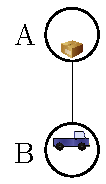
\includegraphics[scale=2]{pdfs/one-truck-one-package.pdf}}
  \raisebox{-0.5\height}{
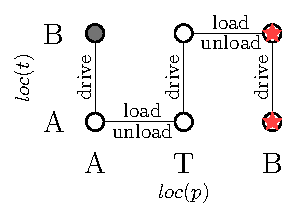
\includegraphics[scale=2]{pdfs/state-space-one-package.pdf}}
  \hspace*{1in}
  \raisebox{-0.5\height}{
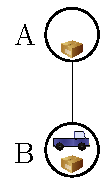
\includegraphics[scale=2]{pdfs/one-truck-two-packages.pdf}}
  \raisebox{-0.5\height}{
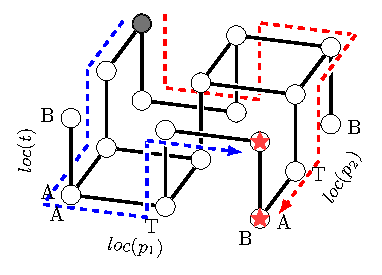
\includegraphics[scale=2]{pdfs/state-space-two-packages.pdf}}
\end{minipage}

\begin{itemize}
\item Optimal planning is to find a plan with the minimal cost.
\item Challenge: \embl{"state explosion problem"}

\end{itemize}
\end{myblock}


\begin{myblock}{Planning as Heuristic Search}
\Large
\begin{itemize}
\item Heuristics: estimations of shortest distance from state to goal
\item Heuristic Search:
\end{itemize}

\begin{minipage}{\textwidth}
  \centering
  \raisebox{-0.5\height}{
\includegraphics[scale=2.5]{pdfs/heuristic-search/{heuristic-search.tikz.preview}.pdf}}
  \raisebox{-0.5\height}{\includegraphics[scale=2.5]{pdfs/heuristic-search/{expanded.tikz.preview}.pdf}}
  \hspace*{0.3in}
  {\LARGE ...}
  \hspace*{0.3in}
  \raisebox{-0.5\height}{\includegraphics[scale=2.5]{pdfs/heuristic-search/{reached.tikz.preview}.pdf}}
\end{minipage}

\begin{itemize}
\item A* with \embl{admissible heuristics} $\rightarrow$ optimal planning
\end{itemize}

\end{myblock}


\begin{myblock}{Abstraction Heuristic}
\Large
\begin{itemize}
\item Abstraction is a mapping from the original state space to an abstract (and much smaller) one.
\item The distances of abstract states to the nearest abstract goal states are used as heuristic values
\end{itemize}

\begin{minipage}{\textwidth}
  \centering
  \raisebox{-0.5\height}{\includegraphics[scale=2.5]{pdfs/abstraction/{abstraction}.pdf}}
  \hspace*{0.5in}
  \raisebox{-0.5\height}{\includegraphics[scale=2.5]{pdfs/abstraction/{arrows}.pdf}}
  \hspace*{0.5in}
  \raisebox{-0.5\height}{\includegraphics[scale=2.5]{pdfs/abstraction/{abstract-space}.pdf}}
\end{minipage}

\begin{itemize}
\item Projection: consider some variables and ignore all others
\end{itemize}

\hspace*{-0.8in}
\begin{minipage}{\textwidth}
  \centering
  \raisebox{-0.5\height}{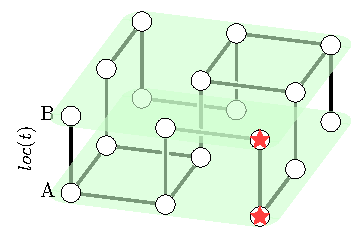
\includegraphics[scale=2.5]{pdfs/abstraction/ignore-packages.pdf}}
  \hspace*{0.1in}
  \raisebox{-0.5\height}{\includegraphics[scale=2.5]{pdfs/abstraction/{ignore-packages-arrow}.pdf}}
  \hspace*{0.5in}
  \raisebox{-0.5\height}{\includegraphics[scale=2.5]{pdfs/abstraction/{ignore-packages-abstract-space}.pdf}}
\end{minipage}

\begin{minipage}{\textwidth}
  \centering
  \raisebox{-0.5\height}{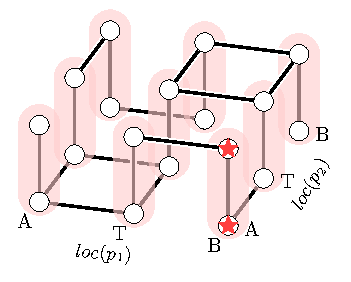
\includegraphics[scale=2.5]{pdfs/abstraction/ignore-truck.pdf}}
  \raisebox{-0.5\height}{\includegraphics[scale=2.5]{pdfs/abstraction/{ignore-truck-arrow}.pdf}}
  \raisebox{-0.5\height}{\includegraphics[scale=2.5]{pdfs/abstraction/{ignore-truck-abstract-space}.pdf}}
\end{minipage}

\end{myblock}

\end{column}

\begin{column}{.32\textwidth}

\begin{myblock}{Merge-and-Shrink}
\Large
\begin{itemize}
\item Merge-and-Shrink (M\&S) transforms the set of \emph{atomic projections} into a flexible abstraction with three operations: \embl{merge}, \embl{shrink} and \embl{label reduction}.
\end{itemize}

\begin{minipage}{0.3\textwidth}
  \centering
  \raisebox{-0.5\height}{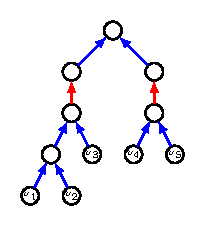
\includegraphics[scale=4]{pdfs/mas/tree.pdf}}
\end{minipage}
\hspace*{1in}
\begin{minipage}{0.5\textwidth}
\begin{algorithm}[H]
\begin{algorithmic}[1]
\STATE $P=\{\text{all atomic projections}\}$
\WHILE{$|P|>=1$}
	\STATE $A_1,A_2=\text{choose-next-merge}(P)$
	\IF{$|A_1|\cdot|A_2|>\text{limit}$}
		\STATE $\text{reduce-labels}(A_1,A_2,S)$
		\STATE $\text{shrink}(A_1,A_2)$
	\ENDIF
\STATE $P=P\cup\{A_1 \otimes A_2\}\setminus\{A_1,A_2\}$
\ENDWHILE
\end{algorithmic}
\caption{Merge-and-Shrink}
\label{alg:seq}
\end{algorithm}

\normalsize
\begin{itemize}
\item which two to merge? $\rightarrow$ merging strategy 
\item how to shrink? $\rightarrow$ shrinking strategy
\item how to reduce labels? $\rightarrow$ label reduction
\end{itemize}
\end{minipage}
\vspace{0.3in}
\begin{itemize}
\item SCC-DFP is the best-performing M\&S in literatures.
\end{itemize}

\end{myblock}

\begin{myblock}{Heuristic Guided Merging Strategy}
\Large
\begin{itemize}
\item The ultimate goal of M\&S is to get a better heuristic.
\item Use \embl{heuristic quality evaluator} to help determine which two abstractions to merge next.
\end{itemize}
\hspace*{1in}
\begin{minipage}{0.8\textwidth}
\begin{itemize}
%\item Evaluate the heuristic quality \embl{improvement} for each pair of abstractions from current pool $S$.
\item \textbf{Q}$_0$ is heuristic on the initial state.
\item \textbf{I}$^+_{\textbf{Q}_0}$ evaluates improvement by comparing \textbf{Q}$_0$ of $A_1 \otimes A_2$ against the sum of \textbf{Q}$_0$ of $A_1$ and $A_2$.
\end{itemize}
\end{minipage}
\vspace*{0.3in}
\begin{itemize}
\item Experiments:
\end{itemize}
\hspace*{0.5in}
\begin{minipage}{0.37\textwidth}
\normalsize
\vspace*{0.3in}
\begin{itemize}
\item IPC benchmarks
\item 39 domains and 1499 tasks
\item 2GB memory / 30 min
\item We compare \embl{coverage} and \embl{number of A* expansions}
\item Results:
\item[\textcolor{blue}{\textbf{+}}] HG solves 36 tasks on which SD fails
\item[\textcolor{red}{\textbf{-}}] but also fails on 26 tasks SD solves
\item[\textcolor{blue}{\textbf{+}}] HG requires fewer expansions than SD in general
\end{itemize}
\end{minipage}
\begin{minipage}{0.57\textwidth}
  \centering
  \raisebox{-0.5\height}{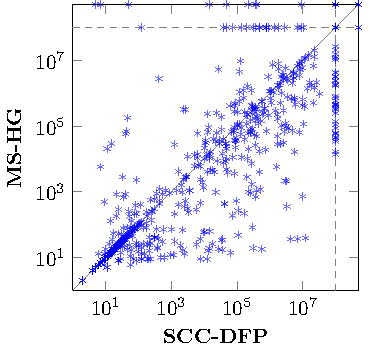
\includegraphics[scale=2.2]{pdfs/figure4.pdf}}
\end{minipage}

\end{myblock}



\begin{myblock}{Issues in Merge-and-Shrink}
\Large
\begin{itemize}
\item M\&S suffers from the expensive construction process:
\end{itemize}

\begin{center}
\begin{minipage}{0.7\textwidth}
\begin{table}
\normalsize 
\centering
\begin{tabular}{|c|c|c|c|c|c|}
\hline\Tstrut
\# Variables & 126 & 169 & 212 & 255 & 298 \\
\hline\Tstrut
 Constr. Time & 157 & 304 & 666 & 1059 & (timeout)\\
\hline
\end{tabular}
\caption{
\normalsize  M\&S construction time (in seconds) on a series of tasks with increasing numbers of variables (atomic projections).}\end{table}
\end{minipage}
\end{center}

\begin{itemize}
\item "passive" shrinking in M\&S is not always the best strategy:
\end{itemize}

\begin{center}
\begin{minipage}{0.7\textwidth}
\begin{table}
\setlength\tabcolsep{5pt}
\centering
\normalsize
\begin{tabular}{|c|c|c|c|c|c|c|}
\hline\Tstrut %\multirow{2}{*}{\hspace{-2pt}\normalsize (b)}
 size limit & MIN & $10^2$ & $10^3$ & $10^4$ & $10^5$ & $10^6$ \\
\hline\Tstrut
 \# expan. & 396 & 9,670 & 21,058 & 44,643 & 14,065 & 9,230 \\
\hline
\end{tabular}
\caption{\normalsize Numbers of nodes expanded by A* using M\&S heuristics constructed with different size limits.}\label{example:2}
\end{table}
\end{minipage}
\end{center}


\end{myblock}


\end{column}

\begin{column}{.32\textwidth}
\begin{myblock}{MS-lite: A Lightweight M\&S}
\Large
\begin{itemize}
\item MS-lite is extremely fast in construction by design:
\end{itemize}

\hspace*{0.5in}
\begin{minipage}{\textwidth}
\begin{itemize}
\item random merge order
\item minimal \embl{$h$-preserving} shrinking
\item no label reduction
\end{itemize}
\end{minipage}

\begin{center}
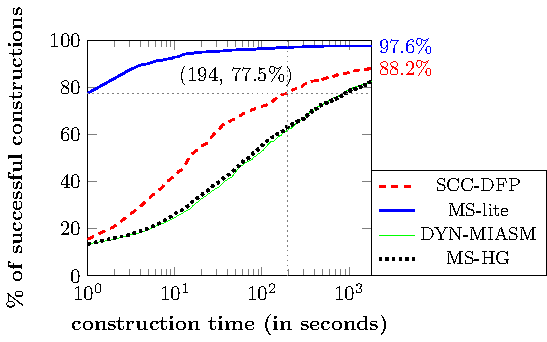
\includegraphics[scale=2.5]{pdfs/time-cdf-figure0.pdf}
\end{center}
%\begin{minipage}{\textwidth}
%  \centering
%  \raisebox{-0.5\height}{}
%\end{minipage}

\begin{itemize}
\item \embl{Complementary strength} of MS-lite:
\end{itemize}

\begin{minipage}{\textwidth}
  \centering
  \raisebox{-0.5\height}{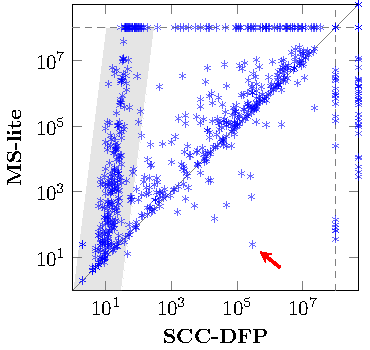
\includegraphics[scale=2.3]{pdfs/figure2.pdf}}
  \hspace*{0.5in}
  \raisebox{-0.5\height}{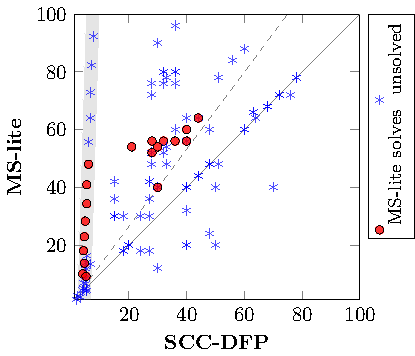
\includegraphics[scale=2.3]{pdfs/figure3.pdf}}
\end{minipage}

\end{myblock}


\begin{myblock}{Combining MS-lite and MS-HG}
\Large
\begin{itemize}
\item Taking maximum of two heuristics, i.e., $h(s)=\max(h_1(s), h_2(s))$, during search.
\item Build MS-lite and another "normal" M\&S, but terminate the construction if it takes too much memory/time.
\end{itemize}


\begin{minipage}{0.45\textwidth}
\begin{itemize}
\item Results:
\end{itemize}
\end{minipage}
\begin{minipage}{0.45\textwidth}
\begin{itemize}
\item Taxonomy:
\end{itemize}
\end{minipage}

\vspace*{0.5in}
\begin{minipage}{0.45\textwidth}
\begin{table}[]
\normalsize
\begin{tabular}{|c|c|c|c|} 
\hline\Tstrut 
 SD & MS-HG & Lite-SD & Lite-HG \\
 \hline\Tstrut 
 \ 671\  & +10 & +47.8 & +75.2 \\
  \hline
 % 718.8$\pm0.5$ & 746.2$\pm0.8$
\end{tabular}
\end{table}
\hspace*{-0.4in}
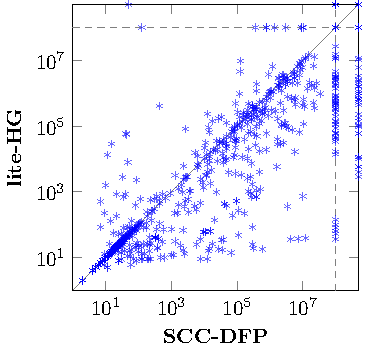
\includegraphics[scale=2.5]{pdfs/figure6.pdf}
\end{minipage}
\begin{minipage}{0.5\textwidth}
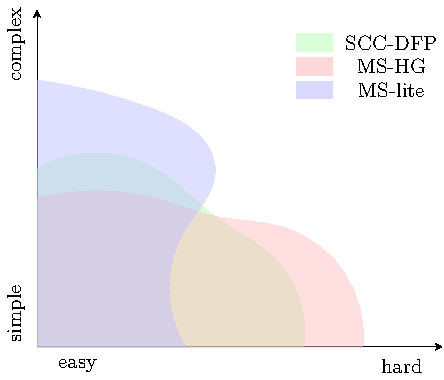
\includegraphics[scale=2.5]{pdfs/taxonomy.pdf}
\normalsize
\begin{itemize}
\item $x$-axis: how hard for state space search?
\item $y$-axis: how complex for creating (M\&S) heuristic?
\end{itemize}
\end{minipage}


\end{myblock}

%\begin{myblock}{Taxonomy}
%\Large
%\begin{itemize}
%\item draw taxonomy \placeholder{1000pt}{600pt}
%\end{itemize}
%
%\end{myblock}



\end{column}

\end{columns}

\end{frame}

\end{document}